%%      VTU Project-report Template using LaTeX
%%      
%%      Copyright 2019 vivek <vivek.adishesha@gmail.com>,
%%	keshav <keshavbharadwaj@gmail.com>
%%      
%%      This program is FREE SOFTWARE; you can redistribute it and/or modify
%%      it under the terms of the GNU General Public License as published by
%%      the Free Software Foundation; either version 2 of the License, or
%%      (at your option) any later version.
%%      
%%      This program is distributed in the hope that it will be useful,
%%      but WITHOUT ANY WARRANTY; without even the implied warranty of
%%      MERCHANTABILITY or FITNESS FOR A PARTICULAR PURPOSE.  See the\include{abstract}
%%      GNU General Public License for more details.
%%      
%%      You should have received a copy of the GNU General Public License
%%      along with this program; if not, write to the Free Software
%%      Foundation, Inc., 51 Franklin Street, Fifth Floor, Boston,
%%      MA 02110-1301, USA.
%
\documentclass[12pt,a4paper,oneside]{memoir}
\usepackage{graphicx}
\usepackage[english]{babel}
\usepackage[a4paper,right=1in]{geometry}
\usepackage{hyperref}
\usepackage{listings}
\usepackage{indentfirst}
\usepackage{caption}
\usepackage{subcaption}
\usepackage{pdfpages}
%\usepackage{subfig}
\usepackage{xcolor}
\usepackage{eso-pic,picture}
\usepackage{float}
\usepackage{amsmath}
\usepackage{background}
\renewcommand{\afterchapternum}{\par\bigskip}
\setlength{\beforechapskip}{-2\baselineskip}
%To reduce%the Chapter vertical height.

%document starts here
\begin{document}
\newlength{\toptafiddle} 
\newlength{\bottafiddle}
\definecolor{rnspurple}{rgb}{0.25,0.04,0.43}
\usetikzlibrary{calc}
\SetBgScale{1}
\SetBgAngle{0}
\SetBgColor{white}
\SetBgOpacity{1}
\SetBgContents							% To apply page borders.
{
	\begin{tikzpicture}[overlay,remember picture]
	\draw [line width=1.5pt]
	($ (current page.north west) + (1.0cm,-1.0cm) $)
	rectangle
	($ (current page.south east) + (-1.0cm,1.0cm) $);
	\end{tikzpicture}
}

\begin{titlingpage}
	%\clearpage
	\thispagestyle{empty}\centering
	\pagecolor{rnspurple}\afterpage{\nopagecolor}
	
\setlength{\toptafiddle}{1in}
\setlength{\bottafiddle}{1in}
\vspace*{-0.75in}
\enlargethispage{\toptafiddle}
\large 
\textbf{\color{white}VISVESVARAYA TECHNOLOGICAL UNIVERSITY\\
	Jnana Sangama, Belagavi - 590 018}\\
\vspace{0.2cm}
\begin{figure}[h]
	\centering
	
\includegraphics[height=3cm]{images/vtu.png}
\end{figure}
\small{\textbf{\color{white}PROJECT REPORT ON}}\\

\Large{\textbf{\color{white}Automated Screening and Health Monitoring System}}\\
\vspace{0.5cm}
\large \textit{\color{white}Thesis submitted in partial fulfillment for the Award of Degree of }{\textbf{\color{white}Bachelor of Engineering}}\\
\color{white} in \\\textbf{\color{white}Electronics and Communication Engineering}
\vspace{0.5cm}\\
{\textbf{\color{white}Submitted by\\}}


\begin{tabular}{lll}
	
\color{white}	Avinash H N & \hspace{5cm} & \color{white}1RN17EC029\\
\color{white}	Karthik A Shet &   & \color{white}1RN17EC066\\
\color{white}	T C Shreyas &   & \color{white}1RN17EC155\\
\color{white}	Kiran Kumar &   & \color{white}1RN17EC066\\
	
\end{tabular}
\vspace{0.5cm}\\
\textit{\color{white}Under the Guidance of}


\Large{\textbf{\color{white} Narendra Kumar}}\\
\textit{\color{white}Assistant Professor}\\

\begin{figure}[h]
	\centering
	
\includegraphics[height=2.7cm]{images/rns1.jpg}
\end{figure}


\begin{center}
	\scriptsize\textbf{\color{white}DEPARTMENT OF ELECTRONICS AND COMMUNICATION ENGINEERING}\\
	\small\textbf{\color{white}(Accredited by NBA for the Academic years 2018-19, 2019-20 and 2020-21)}	
\end{center}
\begin{center}
	\vspace{0.1cm}
	\large\textbf{\color{white}RNS INSTITUTE OF TECHNOLOGY}\\
	\small\textbf{\color{white}(AICTE Approved, VTU Affiliated and NAAC `A' Accredited)\\
		(UG Programs - CSE, ECE, ISE, EIE and EEE have been Accredited by NBA for the Academic years 2018-19, 2019-20 and 2020-2021)\\
		Channasandra, Dr.Vishnuvardhan Road, Bengaluru-560098\\
		2019 - 20}
\end{center}
\end{titlingpage}

%\AddToShipoutPicture{\setlength\fboxsep{8pt}\put(25,25){\framebox(7.65in,11.08in)[lb]{}}}

\begin{titlingpage}
%\clearpage
\thispagestyle{empty}\centering

\setlength{\toptafiddle}{1in}
\setlength{\bottafiddle}{1in}
\vspace*{-1.25in}
\enlargethispage{\toptafiddle}
\large 
\textbf{VISVESVARAYA TECHNOLOGICAL UNIVERSITY\\
	Jnana Sangama, Belagavi - 590 018}\\
\vspace{0.2cm}
\begin{figure}[h]
\centering

\includegraphics[height=3cm]{images/vtu.png}
\end{figure}
{\textbf{PROJECT REPORT ON}}\\

\Huge{\textbf{\color{red} Automated Screening and Health Monitoring System }}
\vspace{0.5cm}

\large \textit{Thesis submitted in partial fulfillment for the award of degree of }{\textbf{Bachelor of Engineering}}\\
in \\\textbf{Electronics and Communication Engineering}
\vspace{0.5cm}\\
{\textbf{Submitted by}}


\begin{tabular}{lll}

Avinash H N & \hspace{5cm}  &1RN17EC029\\
Karthik A Shet &   &1RN17EC060\\
T C Shreyas &   &1RN17EC155\\
Kiran Kumar &   &1RN17EC066\\


\end{tabular}
\vspace{0.5cm}\\
\textit{Under the Guidance of}


\Large{\textbf{Narendra Kumar}}\\
\textit{Assistant Professor}\\

\begin{figure}[h]
	\centering
	
\includegraphics[height=2.5cm]{images/rns1.jpg}
\end{figure}

\begin{center}
\scriptsize\textbf{DEPARTMENT OF ELECTRONICS AND COMMUNICATION ENGINEERING}\\
\small\textbf{(Accredited by NBA for the academic Years 2018-19, 2019-20 and 2020-21)
\\
\vspace{0.5cm}
RNS INSTITUTE OF TECHNOLOGY\\
(AICTE Approved, VTU Affiliated and NAAC `A' credited)\\
(UG Programs - CSE, ECE, ISE, EIE and EEE have been Accredited by NBA for the academic years 2018-19, 2019-20 and 2020-2021)\\
Channasandra,Dr.Vishnuvardhan Road,Bengaluru-560098\\
	 2019-20
}

\end{center}
\end{titlingpage}


%include titlepage,i.e, title.tex file
%Page layout according to VTU specification
%Right=1.25in,left=1in, Top & Bottom 0.75in in each

\setlength{\oddsidemargin}{0.25in}%left side margin{1in by default+0.25in}

%header specification
\setlength{\headheight}{\onelineskip}
\setlength{\headsep}{6pt}
\setlength{\topmargin}{-0.25in}

%footer specification
\setlength{\footskip}{\onelineskip}
\setlength{\footnotesep}{\onelineskip}

%A4 paper height = 11.69in
%thus 11.69in-9.67in-1in(top+header) is approx 0.75in left for bottom
\setlength{\textheight}{9.67in}
\brokenpenalty=10000
\OnehalfSpacing

\include{certificate}
\include{decleration}
\pagenumbering{roman}
\pagestyle{plain}
\include{abstract}
\renewcommand{\abstractname}{Acknowledgement}
\renewcommand{\abstractnamefont}{\Large\textbf}
\renewcommand{\abstracttextfont}{\normalsize}

\begin{abstract}\noindent
\OnehalfSpacing The joy and satisfaction that accompany the successful completion of any task would be incomplete without thanking those who made it possible.
We consider ourselves proud to be a part of RNS Institute of Technology, the institution which molded us in all our endeavors.\\ \\
We express our gratitude to our beloved Chairman \textbf{Dr. R N Shetty} sir, for providing state of art facilities.\\ \\
We express our deep gratitude to \textbf{Dr. H N Shivashankar} sir, Director, who has always been a great source of inspiration.\\ \\
We would like to express our sincere thanks to  \textbf{Dr.M K Venkatesha}, Principal and \textbf{Dr.Vipula Singh} mam, Professor and HOD, Department of E\&CE, for their valuable guidance and encouragement throughout our program.\\ \\
We express our profound gratitude to the coordinators who have given valuable suggestions and guidance throughout the project. We would like to express our sincere gratitude to internal guide \textbf{Narendra Kumar} sir, Assistant Professor for her guidance, continuous support and motivation in completing the project successfully.
We are also thankful to all the teaching and non-teaching faculty of RNSIT for their constant support.

\vspace{2cm}
\begin{flushleft} Avinash H N\\Karthik A Shet\\T C Shreyas\\Kiran Kumar\end{flushleft}
\vfill
\end{abstract}



\setcounter{secnumdepth}{3}%sections numbering upto 3 level
\renewcommand{\contentsname}{Table of Contents}
\tableofcontents
\newpage
\listoffigures
\newpage 
\listoftables


\include{acronyms}

\pagestyle{myheadings}
\makeheadrule{myheadings}{\textwidth}{0.4pt}
\makefootrule{myheadings}{\textwidth}{0.4pt}{\footruleskip}
\makeoddhead{myheadings}{\scriptsize{Automated Screening and Health Monitoring System}}{}{\small{Chapter \thechapter}}
\makeoddfoot{myheadings}{\small{Dept Of ECE, RNSIT, Bengaluru}}{}{\small{\thepage}}

\pagenumbering{arabic}


\index{key}
\chapter{Introduction}
\noindent
In these times of COVID-19 pandemic, there is a high risk of infections at places where there would be gathering of people like schools/colleges, banks, metro stations, malls, sports stadiums, industries, etc. Till the arrival of vaccines/preventive medicines, the spread must be controlled by safety measures like wearing masks, sanitizing hands and maintaining social distancing. At the entrance of every institution/organization, it would be a daunting exercise to manually test everyone’s body temperature, sanitize everyone’s hands and check for masks, as it is not only time consuming, but also involves the risk of infection to the person doing this job. So, there is a dire need for an automated monitoring system. 
Specifically, in the context of educational institutions, there is a need to integrate the attendance monitoring with appropriate screening. The use of touch-based biometrics needs to be avoided.  Thus, our project aims to build an integrated automated screening and health monitoring system, in addition to recording the attendance by facial recognition.
%\section{Problem Statement}
 %To get accurate and meaningful information using CT and MRI images %with minimum error possible

\section{Motivation}
\begin{enumerate}
	\item SOCIAL IMPACT: We want to do a socially relevant project which would help the community for current needs. \par 
	\item PRODUCT DEVELOPMENT:
We also want to do a project which could be commercialized.
 \par
\end{enumerate}

\section{Objectives}
\begin{enumerate}
	\item 	To monitor the temperature of every person entering the institution  \par 
	\item 	To provide warning messages and inform the concerned authorities/health officials for immediate supportive action (via voice or display), for persons with above normal body temperature.\par 
	\item 	To record the attendance via facial recognition algorithm (via voice or display), for persons having normal temperature.\par
	\item 	To check for proper wearing of the mask (via voice or display). \par 
    \item 	To advice the person to use the hand sanitization system (via voice or display), before proceeding further. \par
\item 	To Catalogue all the details of users to the institution database, on a daily basis.\par
\item 	To calculate the Body Mass Index (weight and height ratio) of a person to gauge their fitness. (exact implementation is still under planning)  \par
\item	To use a contactless heart beat sensor for the measurement of pulse/heartbeat. Even this is used to gauge a person’s fitness. (exact implementation is still under planning) \par
\end{enumerate}

\section{Methodology}
\begin{flushleft}
	\textbf{Steps Invloved in Automated Screening and Health Monitoring System} \begin{enumerate}
		\item BODY TEMPERATURE CHECKING - If the temperature of the user is above normal, our system will immediately inform the concerned person/health official.
 
	\item FACIAL RECOGNITION AND MASK MONITORING -ARM Cortex processor which is capable of handling image processing and deep learning algorithms is used.Our health monitoring and screening system has a camera attached to it. With the help of this camera and using the concepts of image processing and deep learning, the attendance of the person is recorded based on facial recognition.Using the same concepts, the system also checks whether the person is wearing the mask or not.

	\item INDICATING THE PARAMETERS - LCD display, LEDs and buzzer are used to indicate parameters of the user like temperature, time of entry, mask detection and name of the person. 

	\item AUTOMATED HAND SANITIZER - Our system also includes, an automated hand sanitizer unit. It has an IR sensor, a DC water pump, transistor and resistors. It is a touch free hand sanitizer dispensing system. This system is independent which works only with DC power supply and not controlled by the ARM processer (as depicted in the block diagram below).
.\end{enumerate}  \end{flushleft}

\section{Applications and Future Scope}
\begin{enumerate}
	\item 	This integrated system can be used at the entrance of educational institutions, metro stations, industries, banks, malls, etc. to screen every individual for his body temperature, mask wearing and hand sanitization. \par 
	\item The system helps in cataloguing the details of users/entrants to an appropriate database \par
 \item 	The system may be made to provide health tips to needy individuals during the leisure time of the system \par
 \item 	The system could be modified to integrate ‘Aarogyasetu App’ as ‘health assistant \par
\end{enumerate}

\begin{figure}[H]
	\centering
	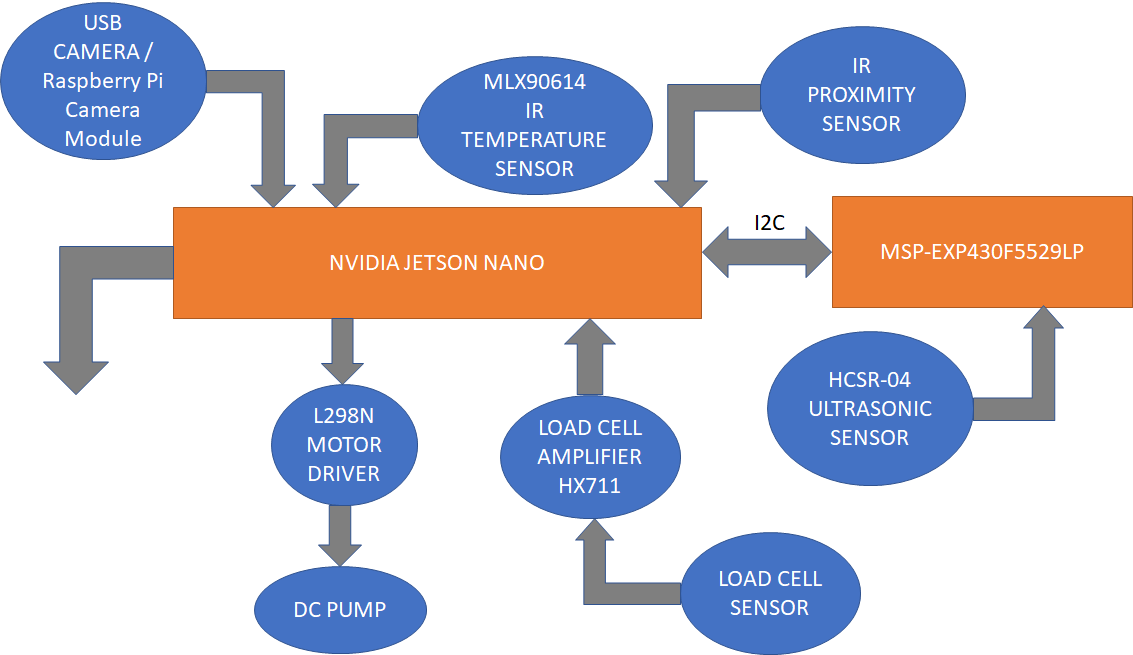
\includegraphics[width=0.7\linewidth]{images/updated bd}
	\caption{Proposed System Block Diagram}
	\label{fig:updated bd}
\end{figure}


		
%\end{flushleft}

\chapter{Literature survey}
\noindent 
\textbf{ARTICLE 1: Design of Automatic Hand Sanitizer System
Compatible with Various Containers}\\
Summary:
This paper suggests the design of an automatic hand sanitizer system compatible
with various sanitizer containers.

Method:When one moves one’s hand close to the device sensor, the hand sanitizer container is pumped once.

Conclusions: The automatic hand sanitizer device proposed in this paper is ultimately expected to contribute to contactless
hand disinfection in public places and virus infection prevention. Additionally, it is economical and eco-friendly by decreasing
waste emissions..\\ \\
%\vspace{0.4cm}
\textbf{ARTICLE 2: Development of a Non-contact Infrared Thermometer by Jing Zhang
School of Energy Engineering, Yulin University, Yulin,719000, China 
}\\
Summary:
It tells the design of Infrared temperature sensor MLX90614 d to collect human or object temperature by the SCM to process the
temperature into the LCD display and alarm when over-temperature. Using software design to complete the control of the system. The smart thermometer can achieve non-contact measurement,
place the thermometer in the forehead for a few seconds to get the body temperature, to alarm once the set value is exceeded. The design temperature range is 0-55 ℃, and temperature resolution is
0.1 ℃.
 \\ \\
%\vspace{0.4cm}
\textbf{ARTICLE 3:ARTICLE 3:Benchmark Analysis of Jetson TX2, Jetson Nano and Raspberry PI using Deep-CNN by Ahmet Ali Süzen, Burhan Duman, Betül Şen.}\\
In this paper Ahmet Ali Süzen et al. have analysed the performance of Jetson TX2, Jetson Nano and Raspberry PI using Deep-CNN.Hardware, low power consumption, high accuracy and performance are crucial factors for deep learning applications.
High level graphics processing units (GPU) are commonly used in high performance deep learning applications.The analysis was done through CNN algorithm created by using fashion product images dataset. 2D CNN model had been developed by Ahmet Ali Süzen et al. so as to classify 13 different fashion products.The Dataset was comprised of 45K pictures. The analysis showed that, the Jetson TX2 had more power consumption, but it performed better in a shorter time, had higher accuracy than others. Jetson TX2 had the highest in cost 399 dollars because low cost is not possible with high hardware features. Raspberry PI without NVIDIA GPU support was the most cost-effective hardware 35 dollars but it was not the right choice for deep learning applications. Since, the hardware which is going to be used in our project should be cost-effective and efficient in terms of its performance, the best choice was Jetson Nano 99 dollars.
\\ \\
%\vspace{0.4cm}
\textbf{ARTICLE 4: “A Real-Time Face Detection Method Using TensorRT and SSD,” Journal of the Korea Information Processing Society: Software and Data Engineering, vol. 9, no. 10, pp. 323–328, Oct. 2020.
  }\\
Summary:Recently, new approaches that significantly improve performance in object detection and recognition using deep learning technology have been proposed. Of the various techniques for object detection, especially facial object detection (Faster R-CNN, R-CNN, YOLO, SSD, etc), SSD is superior in accuracy and speed to other techniques. In this paper, among object detection networks, Mobilenet v2 network is used, models combined with SSDs are trained, and methods for detecting objects. 
Facial object detector was created by H.-B. Yoo et al. as an application to verify the performance of the proposed method, and its behavior and performance were tested in various situations.From this paper, we got the idea of developing our own mask detector on the similar lines.
 \\ \\
 %\vspace{0.4cm}
\textbf{ARTICLE 5: SSD-Mobilenet Implementation for Classifying Fish Species
Phan Duy Hung and Nguyen Ngoc Kien
}\\
Summary:
The objective of this paper was to provide a method to classify fish species automatically via images.The method presented in this paper was a combination of the advantages of both the SSD and Mobilenet models in order to provide the needed high accuracy.
 \\ \\
 %\vspace{0.4cm}
\textbf{ARTICLE 6: "Jetson-inference-pytorch-collect-detection" Github repository
}\\
Summary:
 From this github repository, we understood how to collect our own datasets for object detection on the jetson nano.In our project, the datasets are masked face and unmasked face pictures.

 \\ \\
 %\vspace{0.4cm}
\textbf{ARTICLE 7: ": "Jetson-inference-pytorch-ssd" Github repository
}\\
Summary:
From this github repository, we learnt how to retrain the ssd-mobilenet object detection model to build the proposed mask detection model on the jetson nano.
\\ \\
 %\vspace{0.4cm}
\textbf{ARTICLE 8: "DEVELOPMENT OF AN AUTOMATIC BODY MASS INDEX MACHINE" by Vincent A. Akpan' Joshua B. Agbogun and Oluwatosin T. Omotehinwa
}\\
Summary:
This paper tells about Obesity, which refers to excess body fat in the body, has become a popular and important public health problem. Body mass index 
(BMI) is metric currently in use for defining obesity or anthropometric height/weight characteristics in adults and for classifying them in groups.It is unarguable that rather than error-prone manual BMI calculations, an automatic BMI computation is a preferred option. This paper presents the design and development of a low-cost automatic BMI machine for indoor and out-door use.The performance of the proposed low-cost automatic BMI machine shows that it can be used in homes, hospitals,companies as well as in any environments where routine BMI monitoring may be desired.Recent study conducted among young adults in Nigeria showed that more than one in every 
eight young adults was either overweight or obese.
\\ \\
 %\vspace{0.4cm}
\textbf{ARTICLE 9: "TOUCH LESS HEART BEAT DETECTION WITH CARDIOPULMONARY ANALYSIS" by S.Ushasukanya
, Alladi Saiteja
, Swaroop Duppala
}\\
Summary:
This paper provides a method for communication with fewer pulse regions and a cardiovascular sign
indicating approaches. Using a vector processor, an electromagnetic device at a gap of 1 m from a
human is made to detect the cardiac pulse signal. The suggested method reveals a constraint on the
detection of pulse signals for the reliability of both repeated and strong modulation. Predictions are
carried out at 2.4, 5.8, 10, 16 and 60 GHz, as well as at various power rates between 0 and-27 dBm. In
consideration of the projections developed for both breathing and heart rates, a model for
cardiopulmonary function is described.The pulse rate and the shift in pulse are separated from the
stimulus being provided by wavelets and incredible channels, for SNR between0 and-20 dB.

\\ \\
 %\vspace{0.4cm}
\textbf{ARTICLE 10: "A novel Face Recognition System based on Jetson Nano developer kit" by Thair A. salih and Mohammad Basman Gh
}\\
Summary:
Real-time face recognition became more important in the last two decade, it
is adopted universally for attacking crime, stopping fraud, ensuring public safety.  It
proves that it is one of the most reliable biometrics security systems because frames
can be taken from cameras without touching or interacting, and those images
recorded and spontaneously validated with existing databases. The methodology
achieved in this work will deal with several challenges like real-time recognition,
cheap, portable, and reliable system. NVIDIA Jetson Nano is used in this work. It is
a tiny, powerful AI computer that delivers the estimated performance to run
advanced AI workloads with a small size, low-power, and low-cost.
\\ \\
 %\vspace{0.4cm}
\textbf{ARTICLE 11: "EVM-CNN: Real-Time Contactless Heart Rate
Estimation from Facial Video" by
Ying Qiu, Yang Liu, Juan Arteaga-Falconi, Haiwei Dong
}\\
Summary:
 it was
shown that heart rate information can be extracted from facial
videos by spatial decomposition and temporal filtering. Inspired
by this, a new framework is introduced in this paper for remotely
estimating the heart rate under realistic conditions by combining
spatial and temporal filtering and a convolutional neural network.
 
\include{chapter3}
\include{chapter4}
\include{chapter5}
% \include{Project Code And Results}
\include{conclusion}
\include{reference}
\include{appendix}
\end{document}
